\subsubsection[Separação em Camadas]{Separação em Camadas}

Um dos principios desta restrição está em evitar que clientes façam diretamente requisição para o servidor sem antes passar por um intermediario, como um load balancer ou alguma alguma outra máquina que faça ponte entre servidores. Assegurando que clientes apenas se preocupem com a comunicação, deixando para que intermediários lidem com a distribuição de requisições. \cite{Fielding2000}

\begin{figure}[H]
  \centering
  \resizebox{\columnwidth}{!}{
    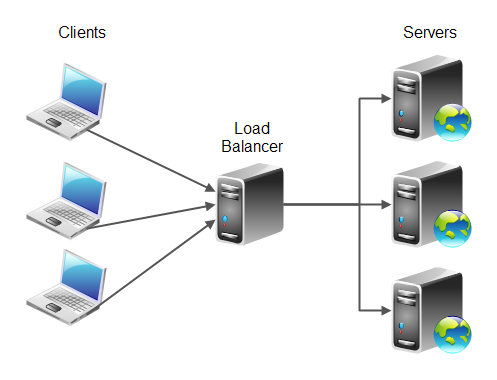
\includegraphics[width=\textwidth,height=\textheight,keepaspectratio]{figuras/load-balancer.png}
  }
  \caption{Exemplo de Load Balancer}
\end{figure}
